\documentclass[a4paper,titlepage]{article}
\usepackage{frontespizio}
\usepackage[english]{babel}
\usepackage[utf8]{inputenc}

\usepackage[a4paper, total={6in, 9in}]{geometry}



\begin{document}
\begin{frontespizio}
\Universita{Verona}
\Dipartimento{Informatica}
\Corso[Laurea]{Informatica}
\Titoletto{Software Engineering}
\Titolo{Second project report}

\Candidato[VR363021]{Giovanni Liboni}
\Candidato[VR359169]{Enrico Giordano}
\Candidato[VR359129]{Alberto Marini}
\Candidato[VR359333]{Alessandro Falda}

\Annoaccademico{2013-2014}
\end{frontespizio}

\tableofcontents

\newpage

\part{Introduction}

This project implements an asynchronous system consists in three principal parts:

\begin{enumerate}

\item a station, that controls velocity of cars;

\item some automatic cars, that set their velocity randomly during the ride and set the ideal velocity thanks to the station;

\item some manual cars, that set their velocity randomly during the ride and receive ``break'' message (but they are not obliged to slow down).

\end{enumerate}

During the execution, is istantiated 50 manual cars and 40 automatic cars and change the speed of each car randomly during the runtime. After a simple ride, the cars decide randomly if they will be exit or not.

\newpage

\part{Graphical interface}

The graphical interface is built with \textit{swing} Java library and consists in two JFrame called ``WallGraphic'' and ``DebugInterface''. The first interface (WallGraphic) is a representation of the situation, composed by a station, some automatic cars and some manual cars. The second interface (DebugInterface) is a textual console that show the program flow, cars display and state and station state. This interface has three option:

\begin{figure}[!h]
\centering
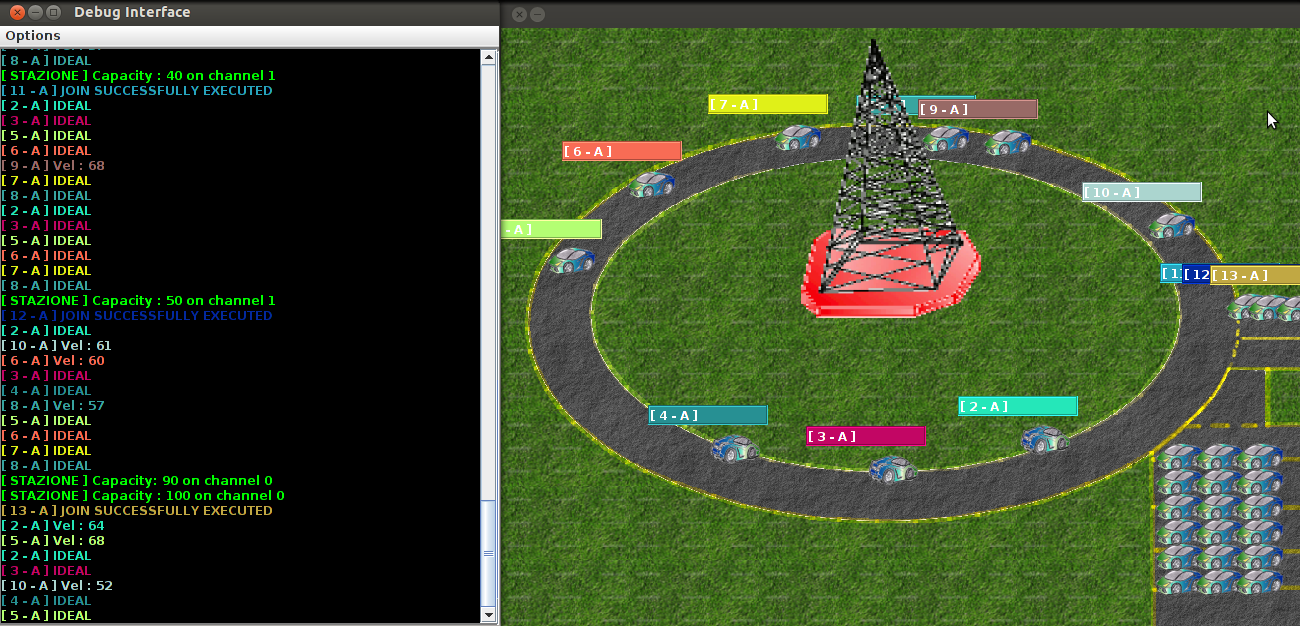
\includegraphics[scale=0.3]{screen.png}
\caption{ScreenShot}
\end{figure}

\begin {enumerate}

\item ``pause'', that stops the program flow acquisition;

\item ``resume'', that resume the program flow acquisition (and enable autoscroll);

\item ``watch'', that disable or enable the autoscroll of the scrollbar.    

\end{enumerate}

Only 200 rows are shown in the screen; after 200 rows, DebugInterface clean itself and delete old rows. This was made because after 200 setText in the same JLabel probably will crash the program.

This is composed by a JFrame that contains a JPanel that contains a JLabel with a black background and a text that was updated by station and cars display.

~

WallGraphic is composed by a JFrame that contains a JPanel with a ``wallpaper'' (the circuit). This JPanel contains in different levels (Z ordered) a station (that is a JLabel with an image) and some cars (that are a JLabels with an image). The cars move theirself in asynchronous way into the ride in 10 different direction (in order to approximate the elliptical path).

The car label have a superior JLabel that contains its id and the car type: the ``M'' letter represent the ``Manual car'' and the ``A'' letter represent the ``Automatic car''. When a car change its direction (X orientation), it changes its image.

\begin{figure}[!h]
\centering
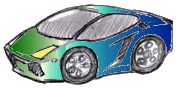
\includegraphics[scale=0.2]{../car.png}
\caption{car label}
\end{figure}


\begin{figure}[!h]
\centering
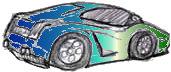
\includegraphics[scale=0.2]{../car2.png}
\caption{car label (different orientation)}
\end{figure}

\begin{figure}[!h]
\centering

\includegraphics[scale=0.5]{../radio.png}
\caption{station label}
\end{figure}


Every car is a graphical thread that execute the move() method in order to move itself during the ride; when a car exit to the circuit, the thread dead. The velocity is graphically represented by a thread sleep during the movement.

~

This is the Z order of the JLabel:

~

~ ~ ~ ~ ~-1: background image;

~

~ ~ ~ ~ ~ 0: station;

~

~ ~ ~ ~ ~-1: cars;

~

In this way, the cars will pass graphically behind the station and on the background image.


In the park, there is a lot of ``dead car'' that simply occupies the park. This was made because is a graphical strategy to fill a space that may seem empty or messy.

~

The graphical class are contained in the \textit{``graphics''} package.

\section{Design pattern for graphical interface}

Every class of this project must use theese graphical interface, so it was implement a \textbf{Façade pattern}. In fact there is a general class, ``ScenarioGraphic'', that include in itself every graphical istance; in this way, when a class must use a graphical istante, simply call the ScenarioGraphic methods and ScenarioGraphic can modify the graphical istances. 

\begin{figure}[!h]
\centering
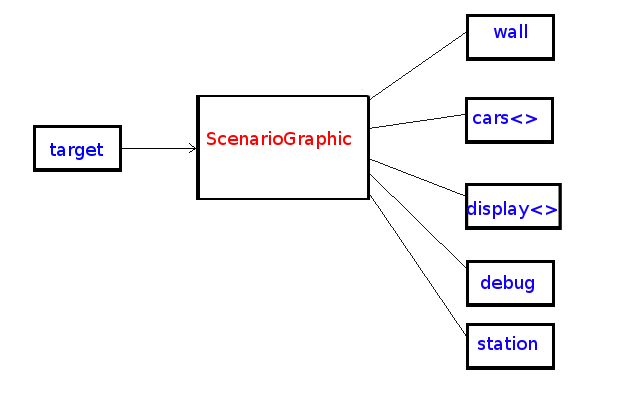
\includegraphics[scale=0.5]{facade.png}
\caption{Façade pattern}
\end{figure}



\section{Swing bug}

The Swing graphical library is a simple and usefull library for java application, but in this project it was used at the limit of its potential. So, every car has two graphic threads that work asynchronously with a fast refresh (20 milliseconds). So, during the execution the GUI may be throws this exception: 

\begin{verbatim}
Exception in thread "Thread-1" java.lang.NullPointerException
	at javax.swing.BufferStrategyPaintManager.flushAccumulatedRegion
	...
\end{verbatim}

This is a bug of Swing library of the management of asynchronous threads that have a very high refresh. But is not important for the program execution, simply is rarely thrown this exception.

\end{document}


